\documentclass[svgnames,11pt]{beamer}
\input{/home/tof/Documents/Cozy/latex-include/preambule_commun.tex}
\input{/home/tof/Documents/Cozy/latex-include/preambule_beamer.tex}
%\usepackage{pgfpages} \setbeameroption{show notes on second screen=left}
\author[]{Christophe Viroulaud}
\title{Tri par tas}
\date{\framebox{\textbf{Algo 09}}}
%\logo{}
\institute{Terminale - NSI}

\begin{document}
\begin{frame}
    \titlepage
\end{frame}
\begin{frame}
    \frametitle{}

    Le tri rapide ou le tri fusion ont une complexité quasi-linéaire ($O(n×\log_2 n)$).
    \begin{framed}
        \centering Peut-on trier efficacement un tableau à l'aide d'un arbre binaire?
    \end{framed}

\end{frame}
\section{Un tas}
\subsection{Définition}
\begin{frame}
    \frametitle{Un tas - Définition}

    Un \textbf{arbre partiellement ordonné} est tel que la valeur de chaque nœud fils est inférieur au nœud père (figure \ref{apo}).
    \begin{center}
        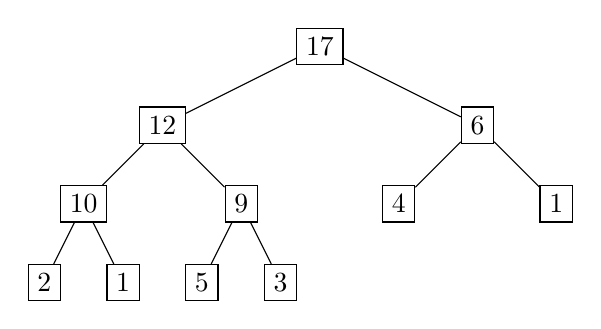
\begin{tikzpicture}
            \node[draw] (0) at (0,0) {17};
            \node[draw] (1) at (-2,-1) {12};
            \node[draw] (2) at (2,-1) {6};
            \node[draw] (3) at (-3,-2) {10};
            \node[draw] (4) at (-1,-2) {9};
            \node[draw] (5) at (1,-2) {4};
            \node[draw] (6) at (3,-2) {1};
            \node[draw] (7) at (-3.5,-3) {2};
            \node[draw] (8) at (-2.5,-3) {1};
            \node[draw] (9) at (-1.5,-3) {5};
            \node[draw] (10) at (-0.5,-3) {3};
            \draw (0) -- (1);
            \draw (0) -- (2);
            \draw (1) -- (3);
            \draw (1) -- (4);
            \draw (2) -- (5);
            \draw (2) -- (6);
            \draw (3) -- (7);
            \draw (3) -- (8);
            \draw (4) -- (9);
            \draw (4) -- (10);
        \end{tikzpicture}
        \captionof{figure}{Arbre partiellement ordonné}
        \label{apo}
    \end{center}

\end{frame}
\begin{frame}[fragile]
    \frametitle{}

    Un \textbf{tas} est un tableau dont l'arbre associé est un arbre partiellement ordonné (code \ref{tas}).

    \begin{center}
        \begin{lstlisting}[language=Python , basicstyle=\ttfamily\small, xleftmargin=2em, xrightmargin=2em]
tas = [17, 12, 6, 10, 9, 4, 1, 2, 1, 5, 3]
\end{lstlisting}
        \captionof{code}{Tas associé à l'arbre \ref{apo}}
        \label{tas}
    \end{center}
    Chaque nœud fils est accessible en respectant la convention suivante:
    \begin{itemize}
        \item l'indice de la racine est 0,
        \item l’indice du fils gauche est 2 ∗ i + 1,
        \item l’indice du fils droit est 2 ∗ i + 2.
    \end{itemize}

\end{frame}
\begin{frame}
    \frametitle{}

    \begin{activite}
        Écrire la fonction \texttt{\textbf{echanger(t: list, i1: int, i2: int)$\;\rightarrow\;$None}} qui inverse les éléments d'indice \textbf{\texttt{i1}} et \textbf{\texttt{i2}} du tableau \textbf{\texttt{t}}.
    \end{activite}

\end{frame}
\begin{frame}
    \frametitle{Avant de regarder la correction}
    \begin{center}
        \centering
        \includegraphics[width=3cm]{/home/tof/Documents/Cozy/latex-include/stop.png}
    \end{center}
    {\Large
    \begin{itemize}
        \item Prendre le temps de réfléchir,
        \item Analyser les messages d'erreur,
        \item Demander au professeur.
    \end{itemize}
    }
\end{frame}
\begin{frame}[fragile]
    \frametitle{Correction}

    \begin{center}
        \begin{lstlisting}[language=Python , basicstyle=\ttfamily\small, xleftmargin=2em, xrightmargin=0em]
def echanger(t: list, i1: int, i2: int) -> None:
    """
    inverse les deux valeurs du tableau
    """
    t[i1], t[i2] = t[i2], t[i1]
\end{lstlisting}
    \end{center}

\end{frame}
\subsection{Tamiser un élément du tableau}
\begin{frame}
    \frametitle{Tamiser un élément du tableau}

    Un tableau n'est pas nécessairement un tas (figure \ref{tamis0}).
    \begin{center}
        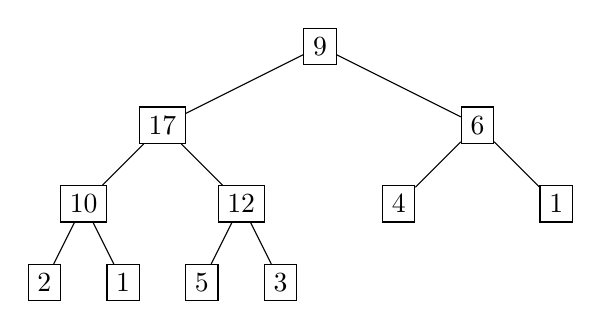
\begin{tikzpicture}
            \node[draw] (0) at (0,0) {9};
            \node[draw] (1) at (-2,-1) {17};
            \node[draw] (2) at (2,-1) {6};
            \node[draw] (3) at (-3,-2) {10};
            \node[draw] (4) at (-1,-2) {12};
            \node[draw] (5) at (1,-2) {4};
            \node[draw] (6) at (3,-2) {1};
            \node[draw] (7) at (-3.5,-3) {2};
            \node[draw] (8) at (-2.5,-3) {1};
            \node[draw] (9) at (-1.5,-3) {5};
            \node[draw] (10) at (-0.5,-3) {3};
            \draw (0) -- (1);
            \draw (0) -- (2);
            \draw (1) -- (3);
            \draw (1) -- (4);
            \draw (2) -- (5);
            \draw (2) -- (6);
            \draw (3) -- (7);
            \draw (3) -- (8);
            \draw (4) -- (9);
            \draw (4) -- (10);
        \end{tikzpicture}
        \captionof{figure}{La racine ne respecte pas les propriétés du tas}
        \label{tamis0}
    \end{center}

\end{frame}
\begin{frame}
    \frametitle{}

    Tamiser un élément du tableau consiste à faire respecter la propriété d'un arbre partiellement ordonné pour ce nœud. Prenons l'exemple du nœud racine contenant la valeur 9. Pour respecter la propriété il faut échanger la valeur du nœud père (9) avec la valeur de son plus grand fils (17).
    \begin{center}
        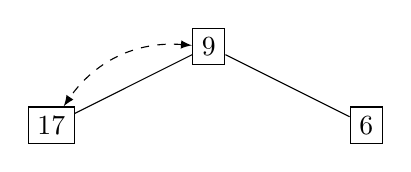
\begin{tikzpicture}
            \node[draw] (0) at (0,0) {9};
            \node[draw] (1) at (-2,-1) {17};
            \node[draw] (2) at (2,-1) {6};
            \draw (0) -- (1);
            \draw (0) -- (2);
            \draw[<->,>=latex,dashed] (0) to[bend right] (1);
        \end{tikzpicture}
        \captionof{figure}{Échange du père avec son plus grand fils.}
        \label{tamis1}
    \end{center}

\end{frame}
\begin{frame}
    \frametitle{}

    \begin{center}
        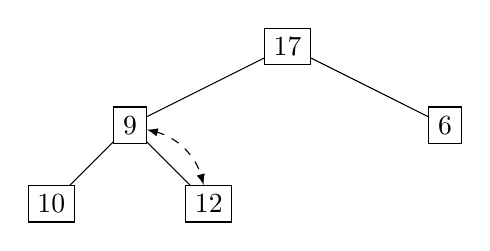
\begin{tikzpicture}
            \node[draw] (0) at (0,0) {17};
            \node[draw] (1) at (-2,-1) {9};
            \node[draw] (2) at (2,-1) {6};
            \node[draw] (3) at (-3,-2) {10};
            \node[draw] (4) at (-1,-2) {12};
            \draw (0) -- (1);
            \draw (0) -- (2);
            \draw (1) -- (3);
            \draw (1) -- (4);
            \draw[<->,>=latex,dashed] (1) to[bend left] (4);
        \end{tikzpicture}
        \captionof{figure}{Propagation récursive}
        \label{tamis2}
    \end{center}

\end{frame}
\begin{frame}
    \frametitle{}

    \begin{center}
        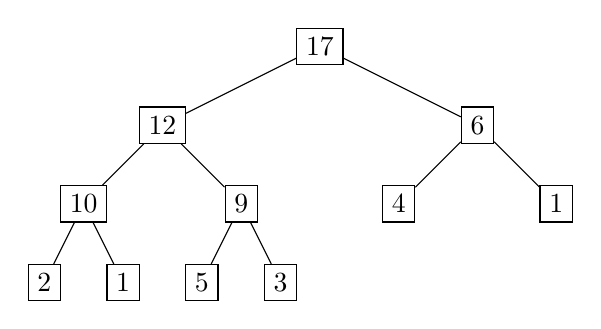
\begin{tikzpicture}
            \node[draw] (0) at (0,0) {17};
            \node[draw] (1) at (-2,-1) {12};
            \node[draw] (2) at (2,-1) {6};
            \node[draw] (3) at (-3,-2) {10};
            \node[draw] (4) at (-1,-2) {9};
            \node[draw] (5) at (1,-2) {4};
            \node[draw] (6) at (3,-2) {1};
            \node[draw] (7) at (-3.5,-3) {2};
            \node[draw] (8) at (-2.5,-3) {1};
            \node[draw] (9) at (-1.5,-3) {5};
            \node[draw] (10) at (-0.5,-3) {3};
            \draw (0) -- (1);
            \draw (0) -- (2);
            \draw (1) -- (3);
            \draw (1) -- (4);
            \draw (2) -- (5);
            \draw (2) -- (6);
            \draw (3) -- (7);
            \draw (3) -- (8);
            \draw (4) -- (9);
            \draw (4) -- (10);
        \end{tikzpicture}
        \captionof{figure}{La valeur 9 est à sa place}
        \label{tamis3}
    \end{center}

\end{frame}
\begin{frame}
    \frametitle{}

    \begin{activite}
        Écrire la fonction \textbf{\texttt{get\_i\_fils\_max(t: list, i\_pere: int, i\_max: int) $\rightarrow$ int}} qui renvoie l'indice du plus grand fils du nœud d'indice \textbf{\texttt{i\_pere}}. Si le père est plus grand que ses fils la fonction renverra \textbf{\texttt{i\_pere}}. De plus la fonction n'ira pas jusqu'au bout du tableau mais s'arrêtera au nœud d'indice \textbf{\texttt{i\_max}} (inclus). Les nœuds suivants seront considérés déjà triés et ne seront plus modifiés.
    \end{activite}

\end{frame}
\begin{frame}
    \frametitle{Avant de regarder la correction}
    \begin{center}
        \centering
        \includegraphics[width=3cm]{/home/tof/Documents/Cozy/latex-include/stop.png}
    \end{center}
    {\Large
    \begin{itemize}
        \item Prendre le temps de réfléchir,
        \item Analyser les messages d'erreur,
        \item Demander au professeur.
    \end{itemize}
    }
\end{frame}
\begin{frame}[fragile]
    \frametitle{Correction}

    \begin{center}
        \begin{lstlisting}[language=Python , basicstyle=\ttfamily\small, xleftmargin=.3em, xrightmargin=-5em]
def get_i_fils_max(t: list, i_pere: int, i_max: int) -> int:
    potentiel = i_pere
    # regarde d'abord le gauche
    i_gauche = 2*i_pere+1
    if i_gauche <= i_max:
        if t[i_gauche] > t[potentiel]:
            potentiel = i_gauche

        # puis le droit
        i_droit = 2*i_pere+2
        if i_droit <= i_max:
            if t[i_droit] > t[potentiel]:
                potentiel = i_droit

    return potentiel
\end{lstlisting}
    \end{center}

\end{frame}
\begin{frame}
    \frametitle{}

    \begin{activite}
        Écrire la fonction récursive \textbf{\texttt{tamiser(t: list, i\_pere: int, i\_max: int) $\rightarrow$ None}} qui respecte l'algorithme suivant:
        \begin{itemize}
            \item Trouver l'indice du nœud maximal entre \textbf{\texttt{i\_pere}} et ses deux fils.
            \item Si l'indice n'est pas \textbf{\texttt{i\_pere}}:
                  \begin{itemize}
                      \item Échanger \textbf{\texttt{i\_pere}} avec son fils le plus grand.
                      \item Tamiser ce nœud fils (qui vient de prendre la valeur de \textbf{\texttt{i\_pere}}).
                  \end{itemize}
        \end{itemize}
    \end{activite}

\end{frame}
\begin{frame}
    \frametitle{Avant de regarder la correction}
    \begin{center}
        \centering
        \includegraphics[width=3cm]{/home/tof/Documents/Cozy/latex-include/stop.png}
    \end{center}
    {\Large
    \begin{itemize}
        \item Prendre le temps de réfléchir,
        \item Analyser les messages d'erreur,
        \item Demander au professeur.
    \end{itemize}
    }
\end{frame}
\begin{frame}[fragile]
    \frametitle{Correction}

    \begin{center}
        \begin{lstlisting}[language=Python , basicstyle=\ttfamily\small, xleftmargin=.5em, xrightmargin=-1em]
def tamiser(t: list, i_pere: int, i_max: int) -> None:
    i_fils_max = get_i_fils_max(t, i_pere, i_max)
    if i_fils_max != i_pere:
        echanger(t, i_pere, i_fils_max)
        tamiser(t, i_fils_max, i_max)
\end{lstlisting}
    \end{center}

\end{frame}
\subsection{Entasser le tableau}
\begin{frame}
    \frametitle{Entasser le tableau}

    En tamisant chaque élément du tableau, on obtient un tas. Une bonne approche est de commencer par le bas de l'arbre. Ainsi, les sous-arbres droit et gauche respectent toujours la propriété d'un arbre partiellement ordonné. De plus, une feuille respectant nécessairement la propriété, il est judicieux de ne commencer qu'au premier nœud qui n'est pas une feuille.

\end{frame}
\begin{frame}
    \frametitle{}

    \begin{activite}
        Écrire la fonction \texttt{\textbf{entasser(t: list)$\;\rightarrow\;$None}} qui transforme le tableau \textbf{\texttt{t}} en tas, en tamisant chaque nœud (qui n'est pas une feuille).
    \end{activite}

\end{frame}
\begin{frame}
    \frametitle{Avant de regarder la correction}
\begin{center}
    \centering
    \includegraphics[width=3cm]{/home/tof/Documents/Cozy/latex-include/stop.png}
    \end{center}
{\Large
    \begin{itemize}
        \item Prendre le temps de réfléchir,
        \item Analyser les messages d'erreur,
        \item Demander au professeur.
    \end{itemize}
}
\end{frame}
\begin{frame}[fragile]
    \frametitle{Correction}

\begin{center}
\begin{lstlisting}[language=Python , basicstyle=\ttfamily\small, xleftmargin=2em, xrightmargin=2em]
def entasser(t: list) -> None:
    # indice du dernier noeud qui n'est pas une feuille
    i = len(t)//2 - 1
    while i >= 0:
        tamiser(t, i, len(t)-1)
        i -= 1
\end{lstlisting}
\end{center}   

\end{frame}
\section{Tri par tas}
\begin{frame}
    \frametitle{Tri par tas}

    Dans un tas la racine contient la plus grande valeur. Il suffit alors d'inverser cette valeur avec la dernière du tableau pour la placer définitivement. Il suffit ensuite d'appliquer le même principe au reste du tableau.
    \begin{center}
    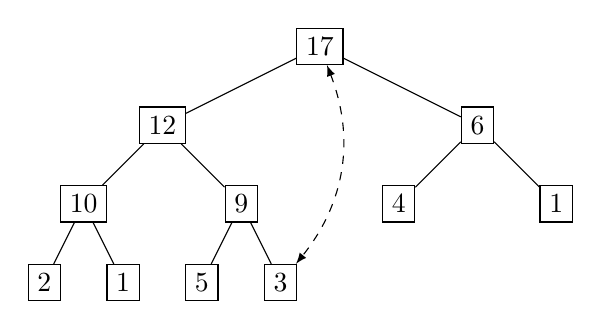
\begin{tikzpicture}
    \node[draw] (0) at (0,0) {17};
    \node[draw] (1) at (-2,-1) {12};
    \node[draw] (2) at (2,-1) {6};
    \node[draw] (3) at (-3,-2) {10};
    \node[draw] (4) at (-1,-2) {9};
    \node[draw] (5) at (1,-2) {4};
    \node[draw] (6) at (3,-2) {1};
    \node[draw] (7) at (-3.5,-3) {2};
    \node[draw] (8) at (-2.5,-3) {1};
    \node[draw] (9) at (-1.5,-3) {5};
    \node[draw] (10) at (-0.5,-3) {3};
    \draw (0) -- (1);
    \draw (0) -- (2);
    \draw (1) -- (3);
    \draw (1) -- (4);
    \draw (2) -- (5);
    \draw (2) -- (6);
    \draw (3) -- (7);
    \draw (3) -- (8);
    \draw (4) -- (9);
    \draw (4) -- (10);
    \draw[<->,>=latex,dashed] (0) to[bend left] (10);
    
    \end{tikzpicture}
    \captionof{figure}{Placer le plus grand élément en fin.}
    \label{apo}
    \end{center}   

\end{frame}
\begin{frame}
    \frametitle{}

    \begin{center}
        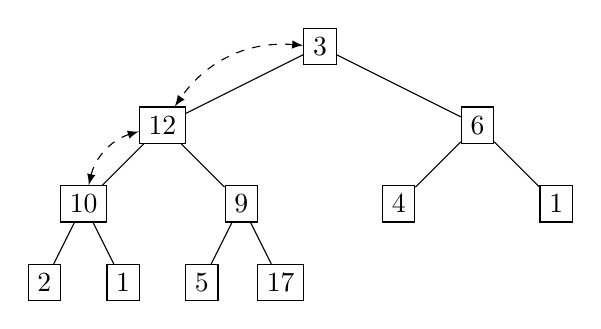
\begin{tikzpicture}
        \node[draw] (0) at (0,0) {3};
        \node[draw] (1) at (-2,-1) {12};
        \node[draw] (2) at (2,-1) {6};
        \node[draw] (3) at (-3,-2) {10};
        \node[draw] (4) at (-1,-2) {9};
        \node[draw] (5) at (1,-2) {4};
        \node[draw] (6) at (3,-2) {1};
        \node[draw] (7) at (-3.5,-3) {2};
        \node[draw] (8) at (-2.5,-3) {1};
        \node[draw] (9) at (-1.5,-3) {5};
        \node[draw] (10) at (-0.5,-3) {17};
        \draw (0) -- (1);
        \draw (0) -- (2);
        \draw (1) -- (3);
        \draw (1) -- (4);
        \draw (2) -- (5);
        \draw (2) -- (6);
        \draw (3) -- (7);
        \draw (3) -- (8);
        \draw (4) -- (9);
        \draw (4) -- (10);
        \draw[<->,>=latex,dashed] (0) to[bend right] (1);
        \draw[<->,>=latex,dashed] (1) to[bend right] (3);
        \end{tikzpicture}
        \captionof{figure}{Tamiser.}
        \label{apo}
        \end{center}

\end{frame}
\begin{frame}
    \frametitle{}

    \begin{center}
        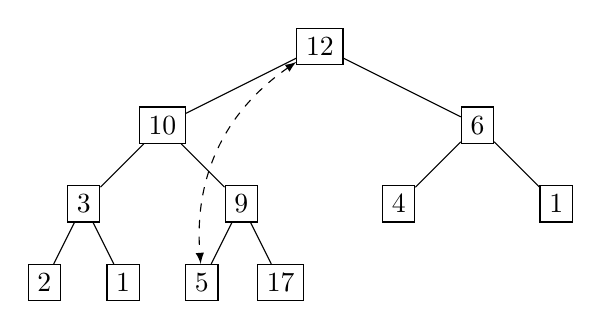
\begin{tikzpicture}
        \node[draw] (0) at (0,0) {12};
        \node[draw] (1) at (-2,-1) {10};
        \node[draw] (2) at (2,-1) {6};
        \node[draw] (3) at (-3,-2) {3};
        \node[draw] (4) at (-1,-2) {9};
        \node[draw] (5) at (1,-2) {4};
        \node[draw] (6) at (3,-2) {1};
        \node[draw] (7) at (-3.5,-3) {2};
        \node[draw] (8) at (-2.5,-3) {1};
        \node[draw] (9) at (-1.5,-3) {5};
        \node[draw] (10) at (-0.5,-3) {17};
        \draw (0) -- (1);
        \draw (0) -- (2);
        \draw (1) -- (3);
        \draw (1) -- (4);
        \draw (2) -- (5);
        \draw (2) -- (6);
        \draw (3) -- (7);
        \draw (3) -- (8);
        \draw (4) -- (9);
        \draw (4) -- (10);
        \draw[<->,>=latex,dashed] (0) to[bend right] (9);
        \end{tikzpicture}
        \captionof{figure}{Recommencer.}
        \label{apo}
        \end{center}

\end{frame}
\begin{frame}
    \frametitle{}

    \begin{activite}
        Écrire la fonction \texttt{\textbf{tri\_par\_tas(t: list)$\;\rightarrow\;$None}} qui implémente l'algorithme suivant:
        \begin{itemize}
        \item Entasser le tableau.
        \item Initialiser \texttt{\textbf{indice\_dernier}}.
        \item Tant que \texttt{\textbf{indice\_dernier}} > 0
        \begin{itemize}
        \item Échanger le premier élément avec l'élément d'indice \texttt{\textbf{indice\_dernier}}.
        \item Tamiser le tableau de la racine jusqu'à l'élément d'indice \texttt{\textbf{indice\_dernier}}.
        \item Décrémenter \texttt{\textbf{indice\_dernier}}.
        \end{itemize}
        \end{itemize}
        \end{activite}

\end{frame}
\begin{frame}
    \frametitle{Avant de regarder la correction}
\begin{center}
    \centering
    \includegraphics[width=3cm]{/home/tof/Documents/Cozy/latex-include/stop.png}
    \end{center}
{\Large
    \begin{itemize}
        \item Prendre le temps de réfléchir,
        \item Analyser les messages d'erreur,
        \item Demander au professeur.
    \end{itemize}
}
\end{frame}
\begin{frame}[fragile]
    \frametitle{Correction}

\begin{center}
\begin{lstlisting}[language=Python , basicstyle=\ttfamily\small, xleftmargin=2em, xrightmargin=2em]
def tri_par_tas(t: list) -> None:
    entasser(t)
    dernier = len(t) - 1
    while dernier > 0:
        echanger(t, 0, dernier)
        tamiser(t, 0, dernier-1)
        dernier -= 1
\end{lstlisting}
\end{center}   

\end{frame}
\begin{frame}[fragile]
    \frametitle{}

\begin{center}
\begin{lstlisting}[language=Python , basicstyle=\ttfamily\small, xleftmargin=2em, xrightmargin=2em]
tab = [randint(0, 100) for _ in range(10)]
print(tab)
tri_par_tas(tab)
print(tab)
\end{lstlisting}
\captionof{code}{Tester la fonction}
\label{CODE}
\end{center}  

\end{frame}
\begin{frame}
    \frametitle{}

    \begin{center}
        Ce tri a une complexité temporelle en $O(n.log(n))$
    \end{center}

\end{frame}
\end{document}